\chapter{Configuración de servicios de red}
Dentro del CNCA se maneja una red particular producto de los diferentes equipos y proyectos que se llevan a cabo. La idea de esta sección es documentar los procedimientos para abrir puertos en el firewall, agregar equipos a la subred adecuada para prestar servicios al público, entre otras cosas esenciales.

\section{Adición de equipos al DHCP y DNS}
Como parte de la expansión del clúster Kabré, así como la prestación de servicios a terceros, entre los cuales se incluye el hosting de equipos, surge la necesidad de manejar de manera centralizada el direccionamiento de puertos y la asignación de direcciones IP. Estas direcciones se administran a través de un servidor DHCP en el nodo meta.cnca y se configura con un cliente de webmin. Para poder acceder a este cliente, se prefiere iniciar una sesión por ssh con exportación de Xorg, y abrir localmente en ese equipo una instancia del navegador web:

\begin{lstlisting}
ssh -X -p22222 usuario@cluster.cenat.ac.cr
firefox &
\end{lstlisting}

Una vez abierto el navegador, ingresamos al sitio \url{http://meta.cnca:10000} e ingresamos las credenciales de root para poder administrar el equipo. Nos aparecerá la pantalla de la figura \ref{fig:dhcp:00}:

En la barra de búsqueda al lado izquierdo, escribimos dhcp y presionamos enter. De las opciones que aparecen, seǵun la figura \ref{fig:dhcp:01}, seleccionamos la primera, la cual nos dirigirá a una pantalla como la mostrada en la figura \ref{fig:dhcp:02}.

\begin{figure}[H]
\centering
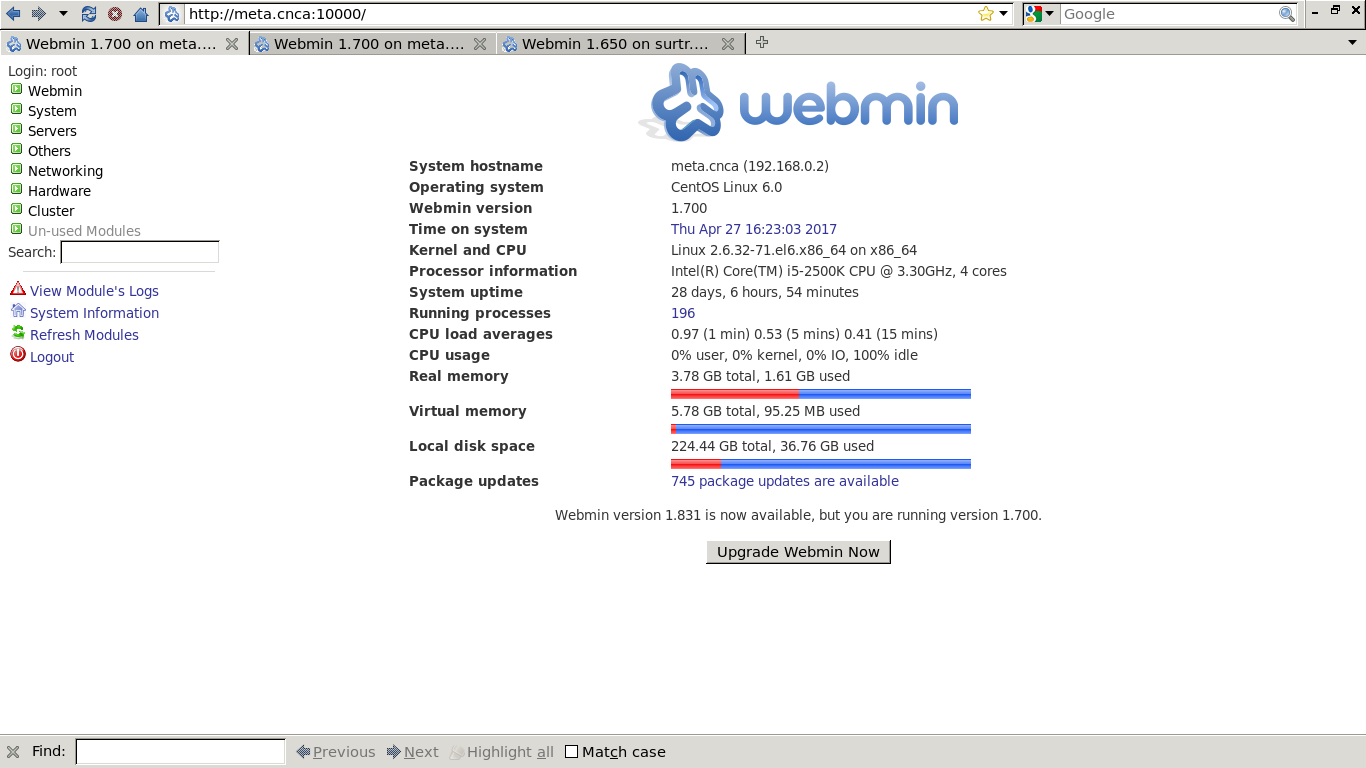
\includegraphics[width=0.70\textwidth]{dhcp00.png}
\caption{Vista inicial de webmin.}
\label{fig:dhcp:00}
\end{figure}

\begin{figure}[H]
\centering
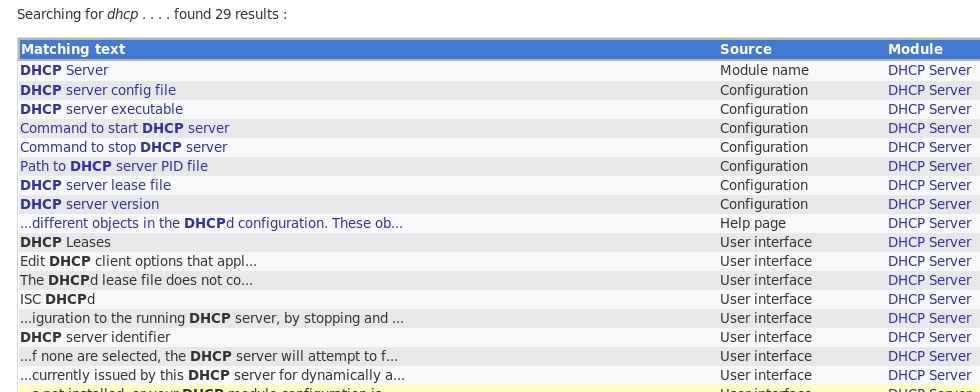
\includegraphics[width=0.70\textwidth]{dhcp01.png}
\caption{Resultados de búsqueda de dhcp.}
\label{fig:dhcp:01}
\end{figure}

\begin{figure}[H]
\centering
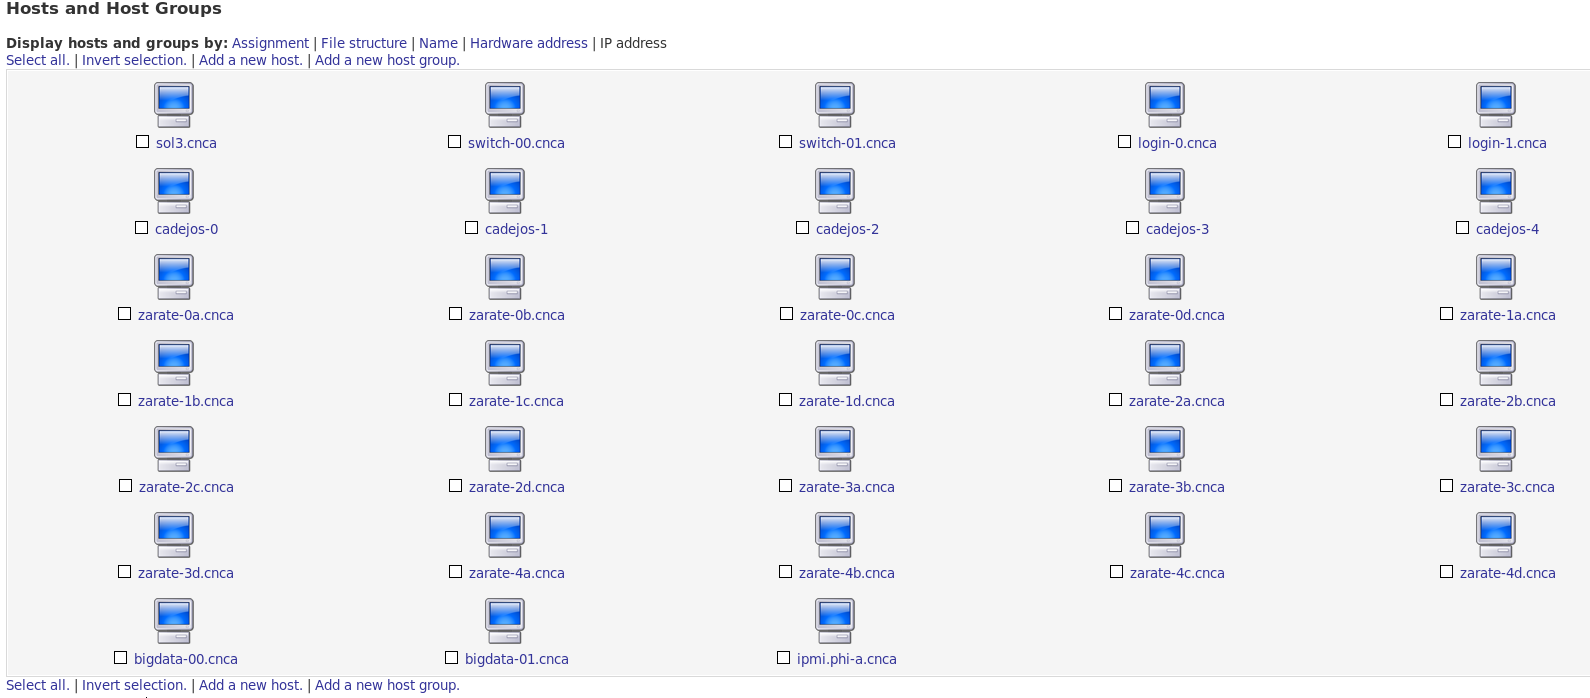
\includegraphics[width=0.70\textwidth]{dhcp02.png}
\caption{Pantalla del servicio DHCP con los hosts agregados actualmente.}
\label{fig:dhcp:02}
\end{figure}

Una vez ubicados en esta pantalla, procedemos a hacer clic en el vínculo Add new host. Esto nos llevará a una pantalla como la mostrada en la figura \ref{fig:dhcp:03}. Basta con especificar los espacios Host name y Fixed IP Address como se muestra en la figura \ref{fig:dhcp:04} para poder agregar el servicio. Luego de esto hacemos clic en Create, y posteriormente nos dirigimos al botón Apply Changes, como se muestra en la figura \ref{fig:dhcp:05} para aplicar los nuevos cambios.

\begin{figure}[H]
\centering
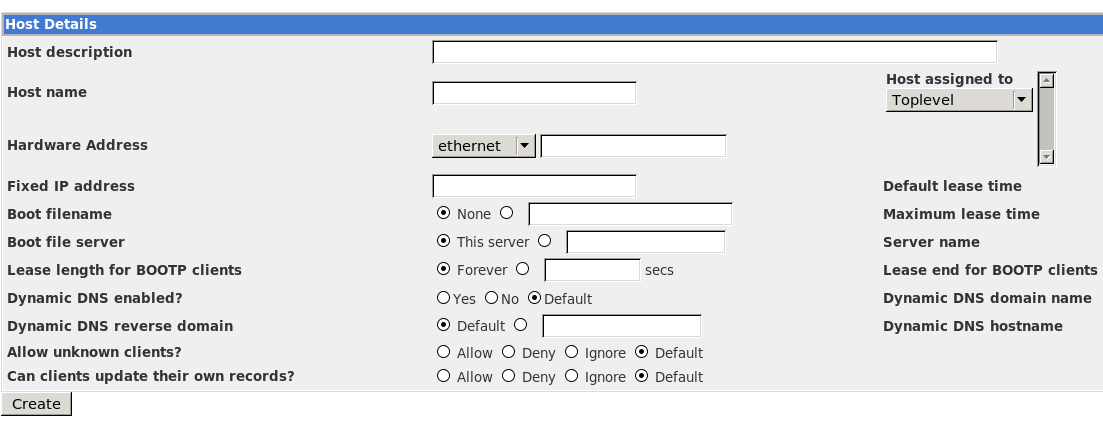
\includegraphics[width=0.70\textwidth]{dhcp03.png}
\caption{Pantalla de adición de host nuevo. Se deben llenar los campos de host name y Fixed IP address.}
\label{fig:dhcp:03}
\end{figure}

\begin{figure}[H]
\centering
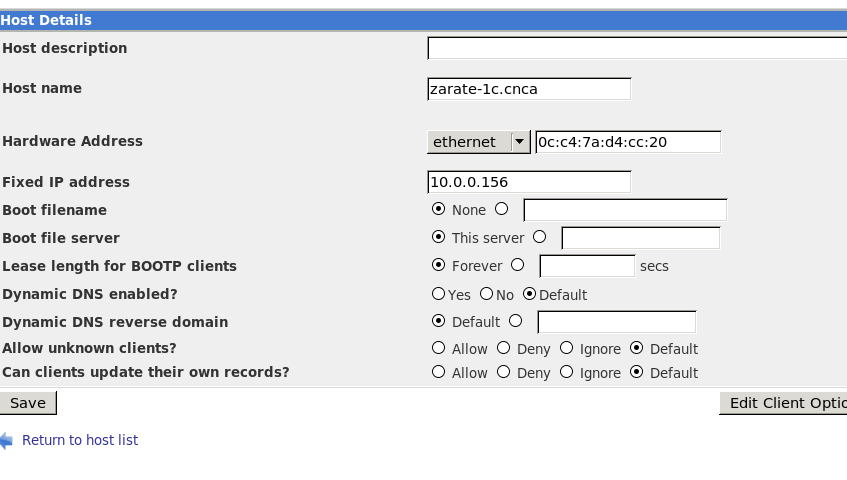
\includegraphics[width=0.70\textwidth]{dhcp04.png}
\caption{Espacios necesarios para poder definir un nuevo host con IP fija.}
\label{fig:dhcp:04}
\end{figure}

\begin{figure}[H]
\centering
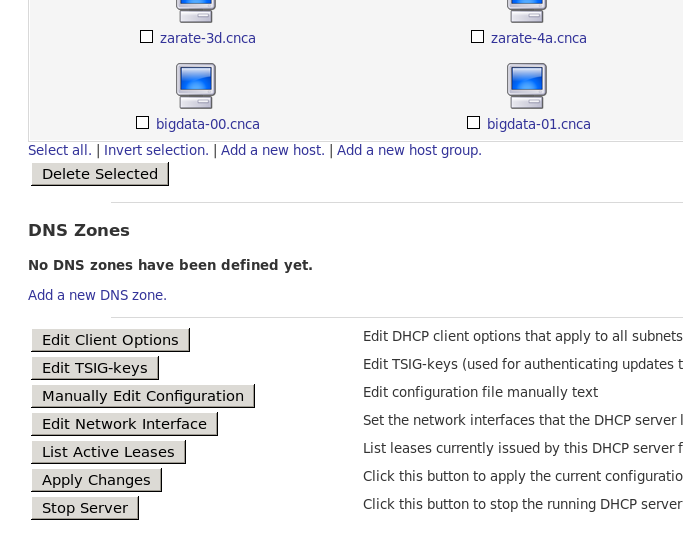
\includegraphics[width=0.70\textwidth]{dhcp05.png}
\caption{Botón de apply changes para que los cambios se reflejen en el servicio.}
\label{fig:dhcp:05}
\end{figure}

Posteriormente a lo anterior, debemos actualizar el DNS. Procedemos a buscar el servicio en la barra de búsqueda lateral, en la cual escribimos DNS y hacemos clic en el primer vínculo, como se muestra en la figura \ref{fig:dns:00}. Esto nos dirige a la pantalla del servicio DNS. A partir de acá nos dirigimos a la sección de zonas DNS y hacemos clic en la zona cnca, mostrada en la figura \ref{fig:dns:01}. 

\begin{figure}[H]
\centering
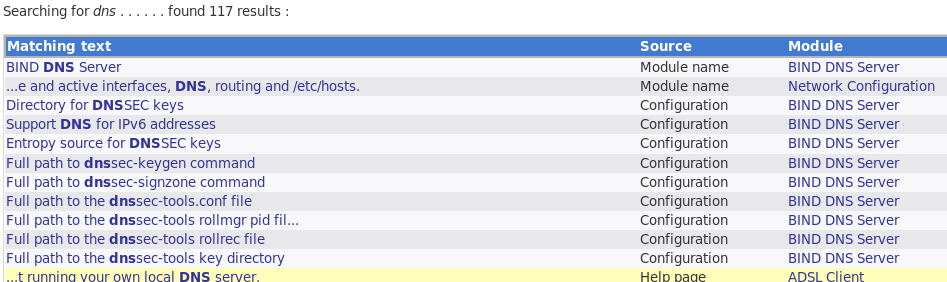
\includegraphics[width=0.70\textwidth]{dns00.png}
\caption{Búsqueda de servicio DNS.}
\label{fig:dns:00}
\end{figure}

\begin{figure}[H]
\centering
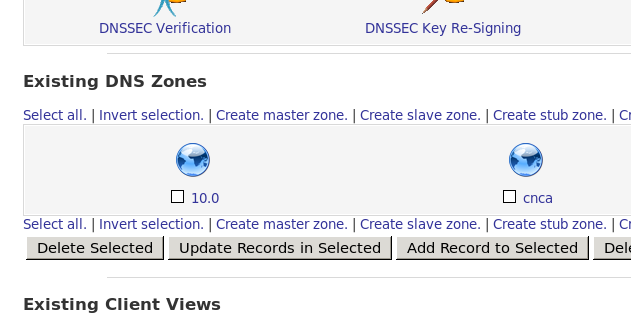
\includegraphics[width=0.70\textwidth]{dns01.png}
\caption{Zonas DNS existentes.}
\label{fig:dns:01}
\end{figure}

En esta sección, hacemos clic en el primer cuadro, el cual dice Address, como se muestra en la figura \ref{fig:dns:02}. Finalmente, estaremos en una pantalla como la de la figura \ref{fig:dns:03} en la cual simplemente agregamos la dirección IP y el host name, y hacemos clic en crear. Nos aseguramos de agregar siempre el dominio .cnca a los hosts.

\begin{figure}[H]
\centering
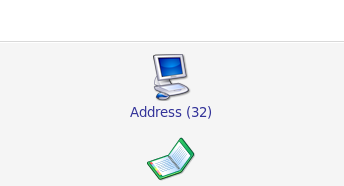
\includegraphics[width=0.70\textwidth]{dns02.png}
\caption{Botón de direcciones pertenecientes a la zona DNS CNCA.}
\label{fig:dns:02}
\end{figure}

\begin{figure}[H]
\centering
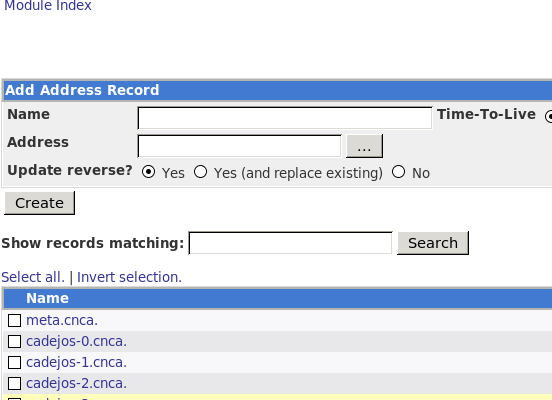
\includegraphics[width=0.70\textwidth]{dns03.png}
\caption{Espacio para agregar equipo nuevo a la zona DNS.}
\label{fig:dns:03}
\end{figure}

\section{Apertura de puertos en el firewall}
En el CNCA es usual que se solicite un espacio en el data center para albergar equipos de centros de investigación de las diferentes universidades públicas. En este caso actualmente se tiene un equipo del TEC (Behemoth), UNA (WRLAA) y uno de la UCR (IDD). Claramente el tener estos equipos implica también habilitar su acceso desde fuera ed la LAN del data center, con lo cual es necesario habilitar nuevas reglas en el firewall surtr, particularmente a nivel de redirección de puertos, los cuales deben además solicitar que se abran a través de un tiquete a CeTIC en el sitio \url{http://intranet.conare.ac.cr/cetic/soporte/open.php}, en el cual se requiere tener una cuenta autorizada. Una vez hecho este trámite, procedemos a redirigir los puertos necesarios. Iniciamos sesión en el meta y abrimos firefox:

\begin{lstlisting}
ssh usuario@cluster.cenat.ac.cr -p22222
firefox
\end{lstlisting}

En el navegador ingresamos a la dirección \url{http://surtr:10000} y en la barra de búsqueda a la izquierda escribimos firewall. de las opciones resultantes nos dirigimos a la primera. Se nos muestra una pantalla como el de la figura \ref{fig:firewall:00}, en la cual nos dirigimos al menú desplegable al lado de botón que dice Showing IPtable, y seleccionamos la tabla Network Address Translation (nat). Esto nos lleva a la pantalla de la figura \ref{fig:firewall:01}, en la cual se muestran las reglas activas. Cabe observar el orden de prioridad de las reglas, pues cualquier regla nueva debe luego ponerse en un nuevo orden de prioridad que no sea de último, pues de este modo se garantiza que funcione (no tiene sentido que una regla de paso o dirección tenga menor prioridad que la de bloqueo, por ejemplo). 

\begin{figure}[H]
\centering
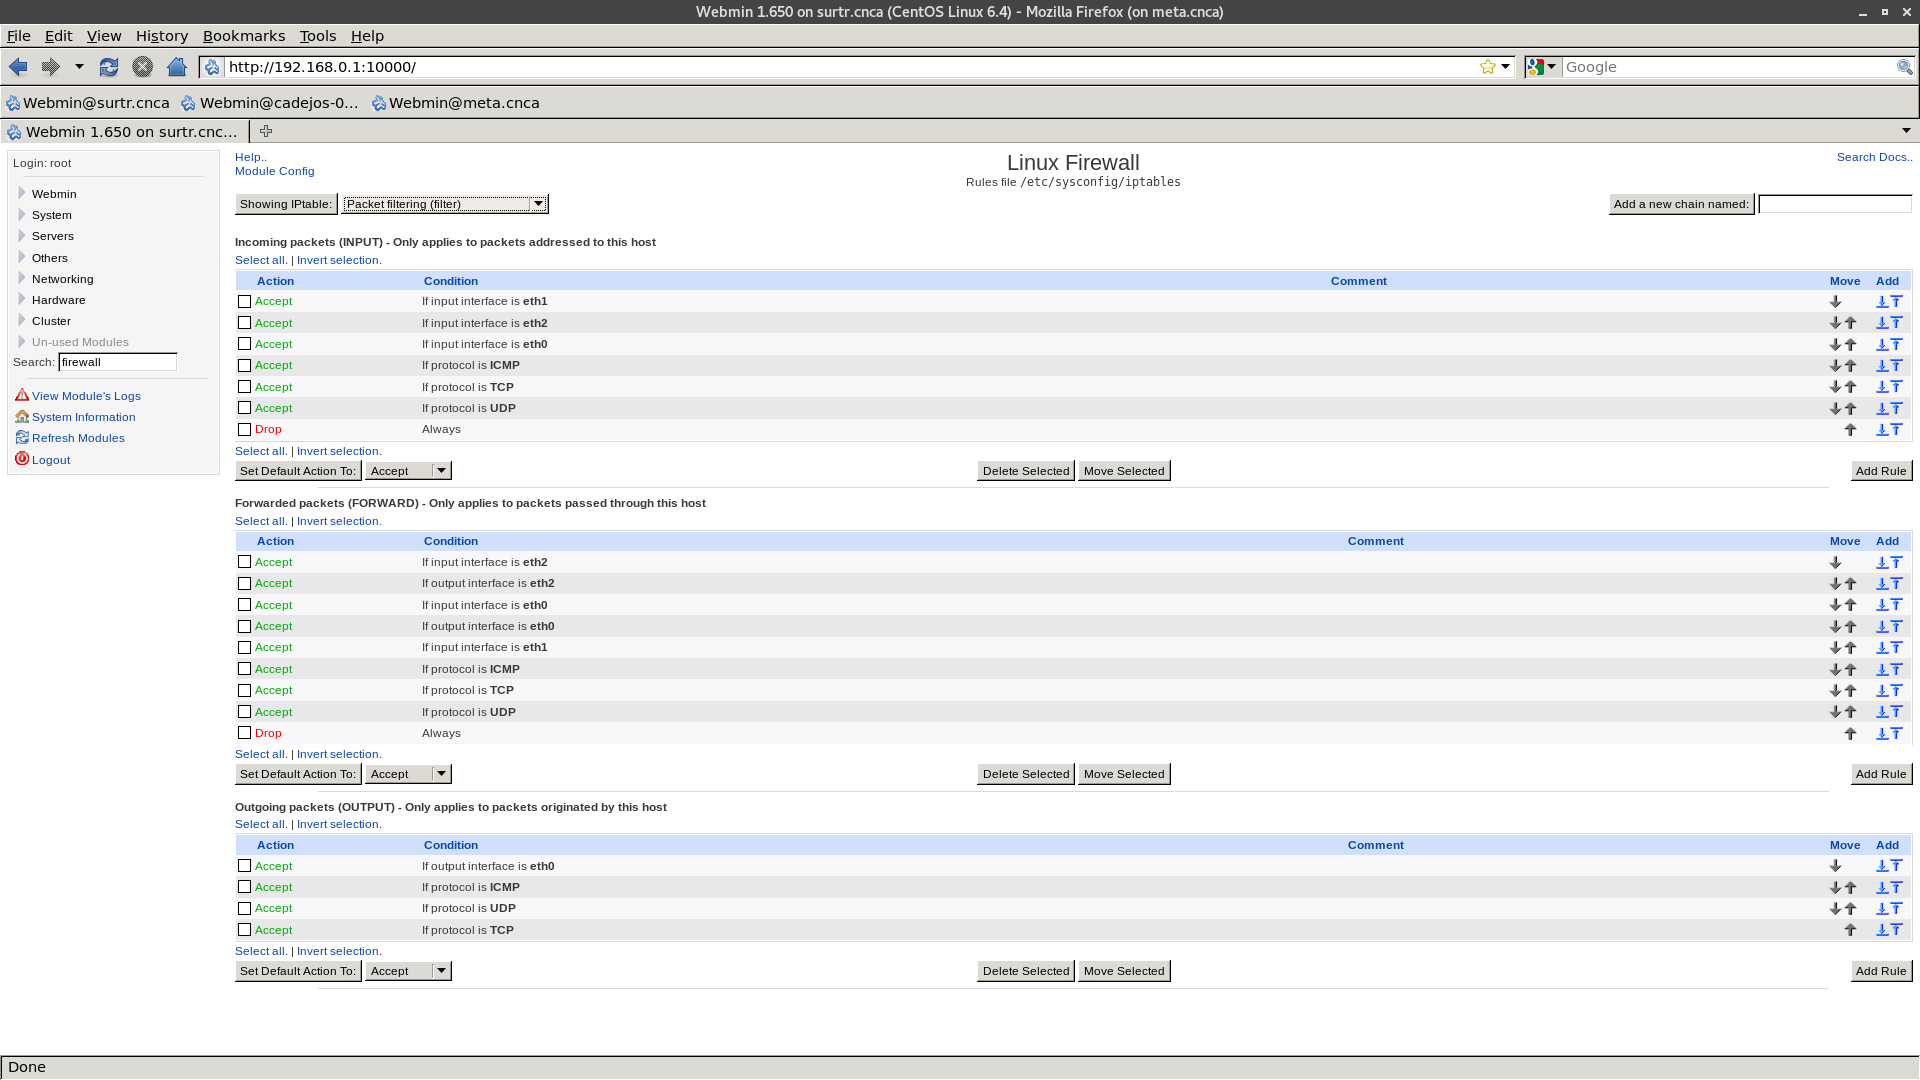
\includegraphics[width=0.70\textwidth]{firewall00.png}
\caption{Espacio para agregar equipo nuevo a la zona DNS.}
\label{fig:firewall:00}
\end{figure}

\begin{figure}[H]
\centering
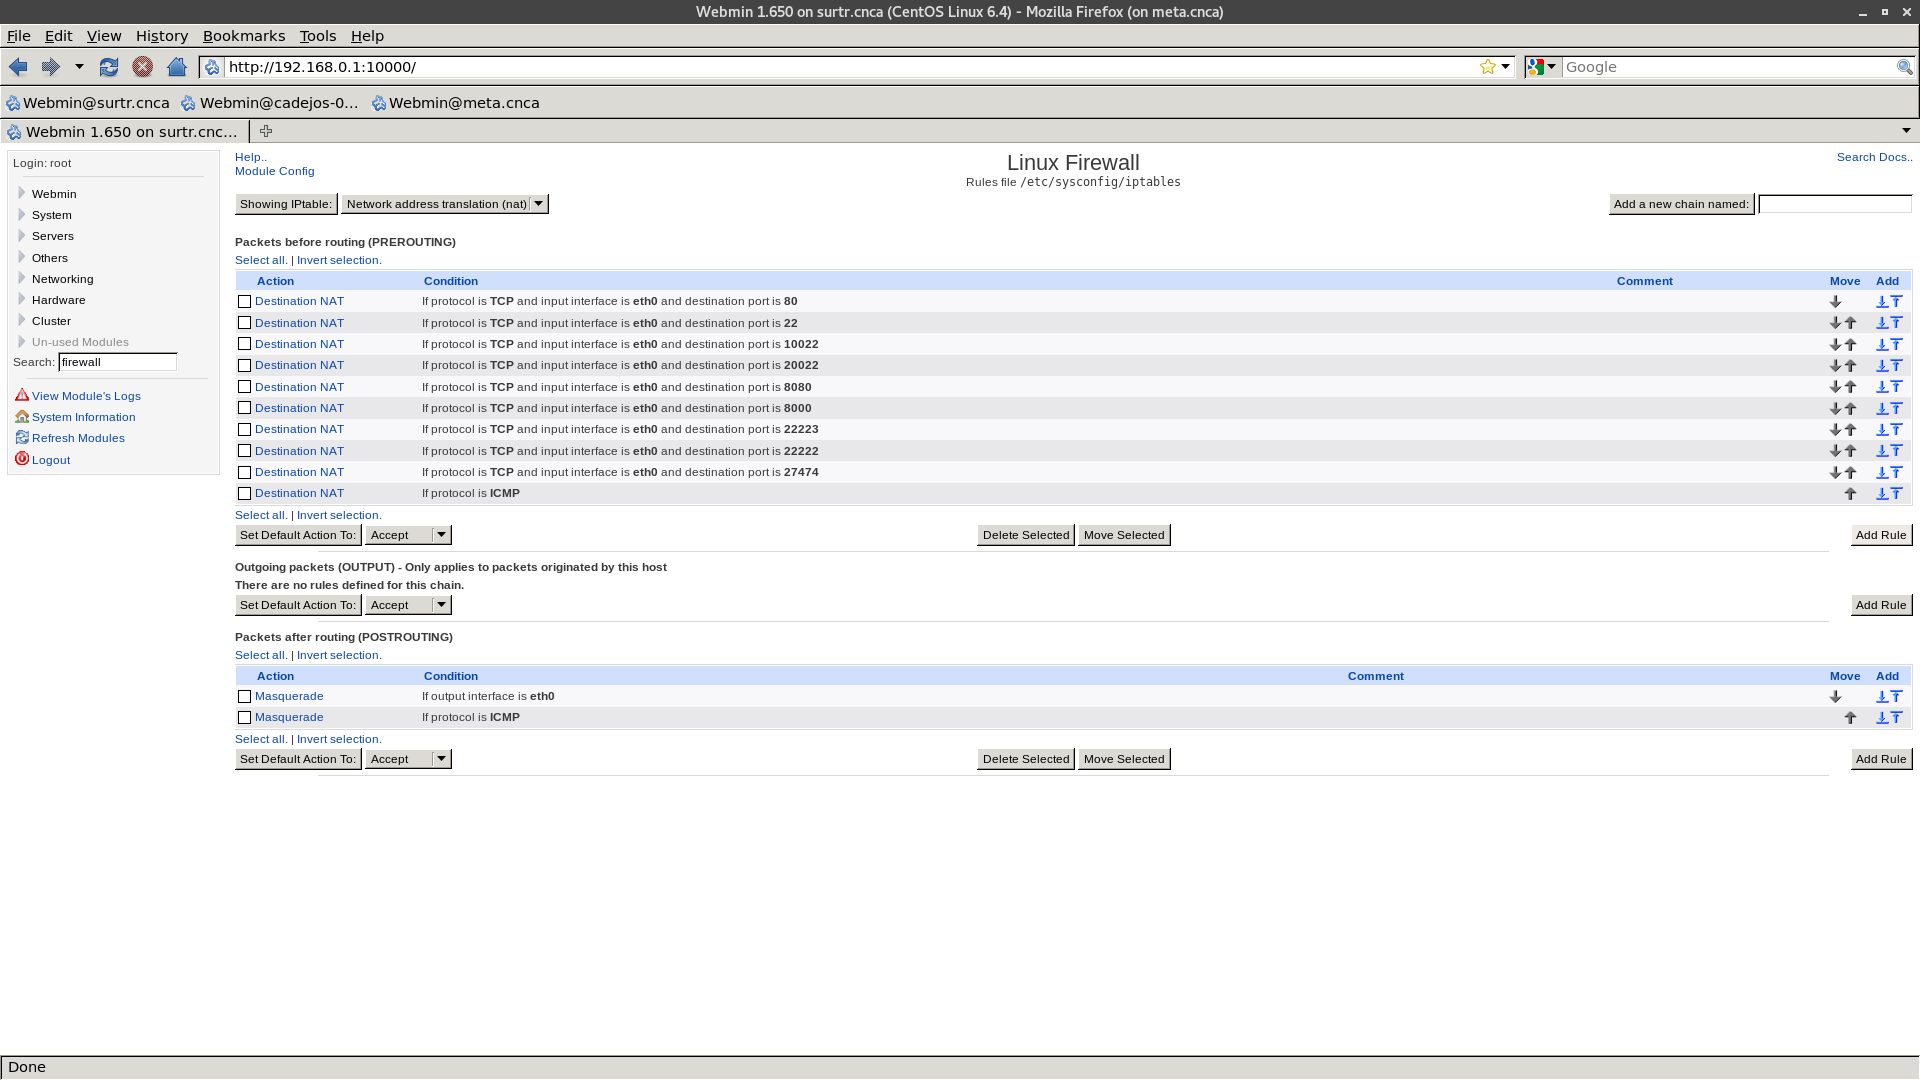
\includegraphics[width=0.70\textwidth]{firewall01.png}
\caption{Espacio para agregar equipo nuevo a la zona DNS.}
\label{fig:firewall:01}
\end{figure}

Al hacer clic en agregar nueva regla, procedemos a llenar los campos correspondientes a la IP del equipo (la cual debe estar en la red 192.168.0.0 y conectado al switch correspondiente) y el puerto de redirección, tal y como se muestra en la figura \ref{fig:firewall:02}. Finalmente salvamos la nueva regla y la reordenamos en la pantalla.

\begin{figure}[H]
\centering
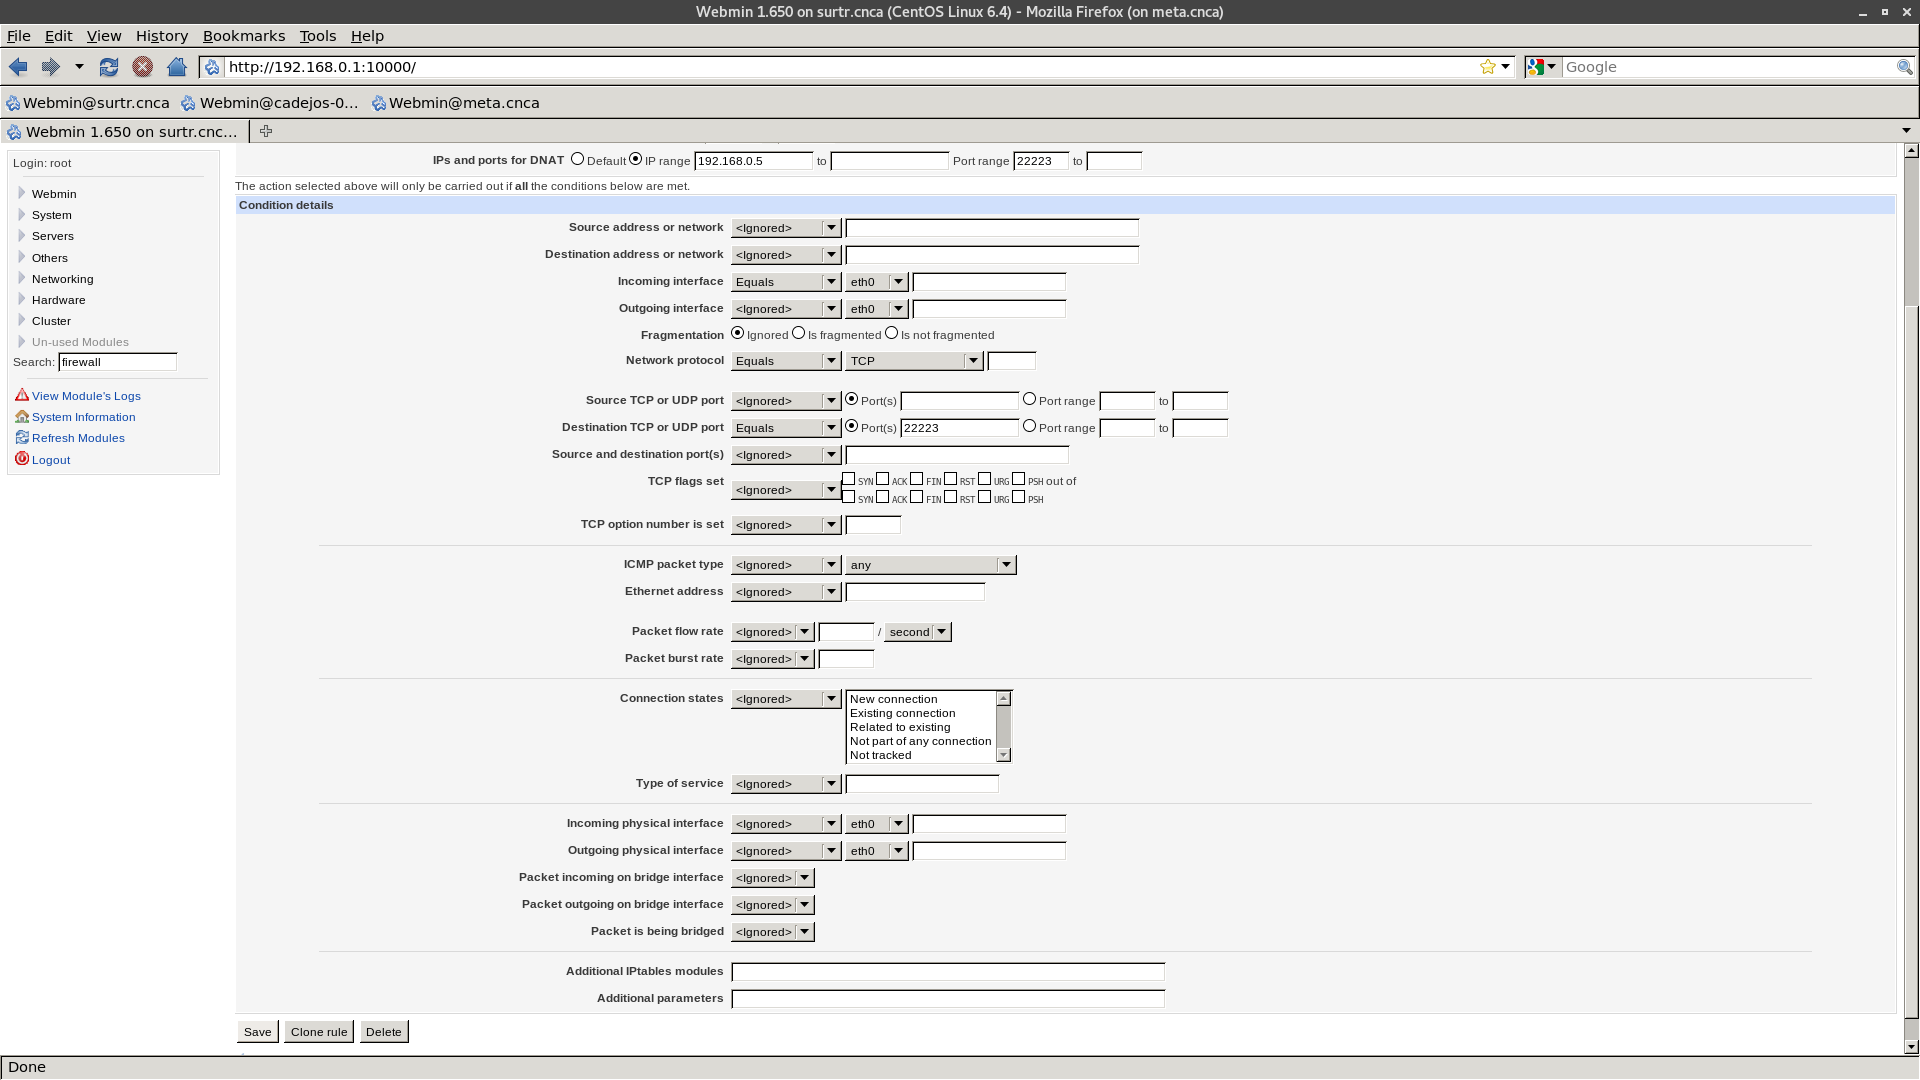
\includegraphics[width=0.70\textwidth]{firewall02.png}
\caption{Espacio para agregar equipo nuevo a la zona DNS.}
\label{fig:firewall:02}
\end{figure}

Cabe mencionar como nota que los equipos agregados a la red 192.168.0.0 se les asigna la IP de forma estática en su configuración local de red. El nodo meta no funciona más que para redirigir los paquetes una vez que estos han pasado a través del firewall.

\subsection{Conservar reglas tras un reinicio en el firewall}
En el servidor surtr, el cual alberga el firewall, suele ser actualizado con nuevas reglas según los servicios que se van agregando a la instalación actual. El detalle está en que iptables no guarda por cuenta propia las reglas nuevas, lo cual provoca que en caso de un reinicio, se deban agregar nuevamente las reglas del firewall \cite{iptables-save}. Para poder salvar dichas reglas, se procede a hacer lo siguiente:

\begin{lstlisting}
chkconfig iptables on
service iptables save
\end{lstlisting}

Lo anterior guarda las reglas en /etc/sysconfig/iptables y propicia que se restauren en cada arranque. Si fuese necesario hacer una restauración manual de las reglas, se puede hacer lo siguiente, asumiendo que hay un respaldo reciente de las reglas:

\begin{lstlisting}
iptables-restore < /etc/sysconfig/iptables
\end{lstlisting}

De igual manera se puede realizar una restauración manual usando una sintaxis similar:

\begin{lstlisting}
iptables-save > /etc/sysconfig/iptables
\end{lstlisting}

\section{VLAN Switch Netgear}

\section{Bonding de puertos}
Esta es una configuración que permite a los equipos habilitados unir de forma lógica diferentes interfaces de red para mejorar la gestión del tráfico de datos y la comunicación en general. No implica estrictamente hablando aumentar el ancho de banda de los puertos, sino la capacidad de mantener varios enlaces simultáneamente con diferentes equipos, al ancho de banda máximo por interfaz. Este procedimiento implica de preferencia contar con interfaces idénticas para ligar (bond), y se debe realizar ajustes a nivel de switch y del nodo específico.
\subsection{Switch Netgear}

\subsection{Nodos}
En cada nodo, se debe cargar el módulo del kernel responsable de gestionar el bonding de puertos a nivel de hardware, no sin antes crear un pequeño archivo de configuración en /etc/modprobe.d/bonding.conf:

\begin{lstlisting}
alias bond0 bonding
options bond0 miimon=100 mode=4 lacp_rate=1
\end{lstlisting}

Lo anterior genera un alias que se referirá al puerto bond0 a crear más adelante, y se le pasan parámetros para el funcionamiento adecuado del enlace. El modo 4 corresponde al estándar IEEE 802.3ad para Dynamic Link Aggregation con protocolos para diferentes anchos de banda, definidos por el parámetro lacp\_rate=1. Ahora cargamos el módulo del kernel:

\begin{lstlisting}
modprobe bonding
\end{lstlisting}

Se procede a crear un archivo de configuración para crear un nuevo puerto llamado bond0 (/etc/sysconfig/network-scripts/ifcfg-bond0) a través , el cual contiene lo siguiente:

\begin{lstlisting}
ONBOOT=yes
DEVICE=bond0
NAME=bond0
TYPE=Bond
BONDING_MASTER=yes
DEFROUTE=yes
BOOTPROTO=dhcp
BONDING_OPTS="mode=4 miimon=100 lacp_rate=1"
\end{lstlisting}

Posteriormente se modifican los archivos de las interfaces que se desea que pertenezcan al bonding (como eth0 y eth1, por ejemplo). Una muestra de configuración sería el siguiente:

\begin{lstlisting}
ONBOOT=yes
HWADDR="0c:c4:7a:d4:f6:8a"
UUID="87c4f9c4-df60-4de7-8ad0-946e71534a41"
BOOTPROTO=none
NAME="eth0"
DEVICE=eth0
TYPE=Ethernet
MASTER=bond0
SLAVE=yes
\end{lstlisting}

Una vez hecho lo anterior, reiniciamos la red.

\begin{lstlisting}
systemctl restart network
\end{lstlisting}

Para el caso particular de sol3, dado que tiene Debian como sistema operativo, se debe modificar únicamente el archivo /etc/network/interfaces con lo siguiente, sin dejar de lado los pasos anteriores para cargar el módulo del kernel.

\begin{lstlisting}
# The loopback network interface
auto lo
iface lo inet loopback
#iface lo inet6 loopback

# eth3 network interface
#auto eth3
#allow-hotplug eth3
#iface eth3 inet dhcp
#    dns-search cnca
#iface eth3 inet6 manual
#    pre-down ip -6 addr flush dev $IFACE

auto bond0
iface bond0 inet static
	address 10.0.0.2
	netmask 255.255.255.0
	network 10.0.0.0
	gateway 10.0.0.1
	slaves eth0 eth1 eth2 eth3 eth4 eth5
	bond_mode 802.3ad
	bond_miimon 100
	bond_downdelay 200
	bond_updelay 200
\end{lstlisting}
Igual que en los casos anteriores, reiniciamos el servicio de red.

\begin{lstlisting}
/etc/init.d/network restart
\end{lstlisting}

\section{Pruebas básicas de ancho de banda}
Iperf es una herramienta utilizada para realizar mediciones de throughput en las conexiones de red \cite{iperf}. Tiene un uso sencillo, el cual se explica a continuación.
\clearpage